% This text is proprietary.
% It's a part of presentation made by myself.
% It may not used commercial.
% The noncommercial use such as private and study is free
% Sep. 2005 
% Author: Sascha Frank 
% University Freiburg 
% www.informatik.uni-freiburg.de/~frank/


\documentclass{beamer}
\usepackage{multirow,multicol}
\usepackage{xcolor}
\makeatletter
\newcommand{\redub}{}
\def\redub#1{%
  \@ifnextchar_%
    {\@redub{#1}}
    {\@latex@warning{Missing argument for \string\redub}\@redub{#1}_{}}%
}
\def\@redub #1_#2{%
    \colorlet{currentcolor}{.}%
    \color{red}%
    \underbrace{\color{currentcolor}#1}_{\color{red}#2}%
    \color{currentcolor}%
}
\makeatother

\newcommand{\gvp}[1]{\textcolor{red}{\ensuremath{#1}}}
\newcommand{\lvp}[1]{\textcolor{blue}{\ensuremath{#1}}}

\begin{document}
\title{Stochastic Variational Inference}   
\subtitle{from Hoffman et al., 2013}
\author{Presented By Ryan Cotterell and Frank Ferraro} 
\date{\today} 

\frame{\titlepage} 

%\frame{\frametitle{Table of contents}\tableofcontents} 

\frame{\frametitle{Overview of Variational Inference}
  \begin{itemize}
    \item Turns a complicated inference problems into an optimization problem
    \item Minimizes the KL divergence from the variational distribution to the posterior
      distribution
    \item EM is a special case
  \end{itemize}
}

\frame{\frametitle{Model Image}
put fig 2 here

give gloss of variables: relate them to the input/output/nuissance ones Jason defines
}

\frame{\frametitle{Evidence Lower Bound (ELBO)}
  \begin{itemize}
    \item Key insight is the use of Jensen's inequality
    \item We choose $q$ from some family of distributions $\mathcal{Q}$
  \end{itemize}

  \begin{eqnarray*} %% Do avoid eqnarray if possible.
    \log(p(x \mid \alpha)) & = & \log \int p(x,z,\beta \mid \alpha) dz \ d\beta \\
    \uncover<2->{& = & \log \int p(x,z,\beta \mid \alpha) \frac{q(z,\beta)}{q(z,\beta)} dz d\beta \\}
    \uncover<3->{& = & \log\left(\mathbb{E}_q \left[ \frac{p(x,z,\beta \mid \alpha)}{q(z,\beta)} \right] \right) \\}
    \uncover<4->{& \geq & \mathbb{E}_q \left[ \log p(x,z,\beta \mid \alpha)\right] - \mathbb{E}_q \left[ q(z,\beta) \right] \\}
    \uncover<5->{& = & \mathcal{L}(q)}
  \end{eqnarray*}
}

\frame{\frametitle{Why does maximizes the ELBO minimize the KL-Divergence?} 
  \begin{eqnarray*} %% Do avoid eqnarray if possible.
    \text{KL}(q(z,\beta)||p(z,\beta|x) &=& \mathbb{E}_q \left[ \log(q(z,\beta) \right] - \mathbb{E}_q 
\left[ \log p(z,\beta|x) \right] \\
    & = & \mathbb{E}_q \left[ \log(q(z,\beta) \right] - \mathbb{E}_q 
\left[ \log p(z,\beta,x) \right] + \log p(x) \\
    & = & -\mathcal{L}(q) + const.
    \end{eqnarray*}
    
    \begin{itemize}
      \item Maximizing $\mathcal{L}(q)$ is just minimizing $-\mathcal{L}(q)$
    \end{itemize}

}


\frame{\frametitle{Common Distributions}
\begin{block}{}
\begin{enumerate}
\item Dirichlet

\indent $p(x\ \mid\ \alpha) = \dfrac{\Gamma(\sum \alpha_i)}{\prod \Gamma(\alpha_i)} \prod x_i^{\alpha_i - 1}$
\item Categorical

\indent $p(x\ \mid\ \mathbf{p}) = \prod p_i^{1[x = i]}$
\item Gaussian

\indent $p(x\ \mid\ \mu,\sigma^2) = \dfrac{1}{\sigma \sqrt{2\pi}} \exp{\left( -\dfrac{(x-\mu)^2}{2\sigma^2}\right)}$
\end{enumerate}
\end{block}

\uncover<2->{
\begin{block}{}
\begin{center}
$p(x\ \mid\ \alpha) = 
\alt<3->{\redub{h(x)}_{Support}}{h(x)}
\exp{
	\left( 
\alt<4->{\redub{\theta}_{\textrm{Natural Parameters}}}{\theta} \cdot 
\alt<5->{\redub{T(x)}_{\textrm{Sufficient Statistics}}}{T(x)} - 
\alt<6->{\redub{A(\theta)}_{\textrm{Log Normalizer}}}{A(\theta)}
\right)
}$
\end{center}
\end{block}
}
}

\frame{\frametitle{Common Distributions \ldots in Canonical Form}
\begin{block}{}
\begin{enumerate}
\item Dirichlet
\begin{itemize}
\item $\theta = 
\left(
\begin{array}{c}
\alpha_i - 1
\end{array}
\right)_i$ , 
 $T(x) = 
\left(
\begin{array}{c}
\log x_i
\end{array}
\right)_i
$
\end{itemize}
\item Categorical
\begin{itemize}
\item $\theta = 
\left(
\begin{array}{c}
\log p_i
\end{array}
\right)_i$ , 
 $T(x) = 
\left(
\begin{array}{c}
1[x_j = i]
\end{array}
\right)_i
$
\end{itemize}
\item Gaussian
\begin{itemize}
\item $\theta = 
\left(
\begin{array}{c}
\frac{\mu}{\sigma^2} \\
\frac{-1}{2\sigma^2}
\end{array}
\right)$ , 
 $T(x) = 
\left(
\begin{array}{c}
x \\
x^2
\end{array}
\right)
$
\end{itemize}
\end{enumerate}
\end{block}

\begin{block}{}
\begin{center}
$p(x\ \mid\ \alpha) = \redub{h(x)}_{Support}
\exp{
	\left( 
\redub{\theta}_{\textrm{Natural Parameters}} \cdot 
\redub{T(x)}_{\textrm{Sufficient Statistics}} - 
\redub{A(\theta)}_{\textrm{Log Normalizer}}
\right)
}$
\end{center}
\end{block}
}

\frame{\frametitle{Useful properties of log partition, $A(\theta)$}
\begin{enumerate}
\item $\nabla_\theta A(\theta) = \mathbb{E}_q[ T(x)]$
\item<2-> $\nabla_\theta^2 A(\theta) = \text{Fisher information matrix}$
\end{enumerate}
}

\frame{\frametitle{Coordinate ascent mean-field variational inference}
\begin{enumerate}
\item Mean-field: each latent variable is independent
\begin{align*}
q(z, \beta) = q_{ \alt<2->{\gvp{\lambda}}{\lambda}}(\beta)
\prod_{n=1}^N \prod_{j=1}^J
q_{ \alt<2->{\lvp{\phi_{n,j}}}{\phi_{n,j}}}(z_{n,j})
\end{align*}
\begin{itemize}
\item<3-> Entropy decomposes 
\end{itemize}
\item<4-> Assume $q_{ \text{variational params}}(\cdot)$ is in (the same) exponential family as $p$
\begin{itemize}
\item<5-> $\lambda$ and $\phi_{n,j}$ are the \textit{natural (variational) parameters}
\item<6-> Individual expectations are ``simple'' to compute
\end{itemize}
\item<7-> The posterior (global) natural parameters under $p$ are 

$$\eta_g(x,z,\alpha) = \left( \alpha_1 + \sum_{n=1}^N T(z_n,x_n), \alpha_2 + N\right)$$
\end{enumerate}
}

\frame{\frametitle{Mean Field ELBO}
\begin{enumerate}
\item Since entropy decomposes as
$
\mathbb{E}_q[\log q(z,\beta)] = \mathbb{E}_\lambda[\log q(\beta)] + \sum_{n,j} \mathbb{E}_{\phi_{n,j}}[\log q(z_{n,j})],
$
\item<2-> And $p(x,z,\beta) = p(x,z) p(\beta | x,z)$
\item[]<3->
\begin{align*}
\mathcal{L}(\gvp{\lambda}) 
& = & \mathbb{E}_q [\log p(\beta, x, z)] - \mathbb{E}_q [ \log q(z,\beta)] + C_0 \\
\uncover<4->{& = & \mathbb{E}_q [\log p(\beta | x, z)] - \mathbb{E}_q [ \log q(\beta)] + C_1} \\ \\
\uncover<5->{
\nabla_\lambda \mathcal{L}(\gvp{\lambda}) 
& = & \nabla_\lambda^2 A_g(\lambda) \left(\mathbb{E}_q[ \eta_g(x,z,\alpha)] - \lambda\right)\\
}
\end{align*}
\item<6-> 
$\alt<7->{\redub{\lambda}_{\text{Variational}}}{\lambda} 
= \alt<9->{\redub{\mathbb{E}_q}_{\text{Under Variational}}}{\mathbb{E}_q} [ 
\alt<8->{\redub{\eta_g (x,z,\alpha)}_{\text{Original}}}{\eta_g (x,z,\alpha)}
]$
\item<10-> A similar update exists for the local parameters \lvp{\phi_{n,j}}

$$\phi_{n,j} 
= \mathbb{E}_q [ \eta_l (x_n,z_{n,\backslash j},\alpha) ]
$$
\end{enumerate}
}

\frame{\frametitle{How is EM a special case?}
  \begin{itemize}
    \item How do we choose $\mathcal{Q}$?
    \item We want it to be easily computable!
    \item What if $p(z,\theta |x) \in \mathcal{Q}$? 
    \item Then computing expectations under $q$ is just inference
      in our model!
    \item Consider a standard HMM, our E-step involves direct computation of the marginals through Forward-Backwards
    \item Let $p_\theta(z|x)$ be our model and $\theta_1$ be a setting of parameters
      where $z$ is a latent variable (tags in an HMM) and $x$ is an observed variable (words in an HMM)
    \item Since $p_\theta \in \mathcal{Q},\; \forall \theta \in \Theta$, we simply need to maximize
      $\sum_z p(z|x;\theta_1) \log\left(p(z|x; \theta_2)\right)$ with respect to $\theta_2$
  \end{itemize}
  

}
 

\frame{\frametitle{Low Euclidean distance $\neq$ low distribution similarity}
\begin{itemize}
\item $p_1 \sim \mathcal{N}(\mu_1,\sigma_1)$, $p_2 \sim \mathcal{N}(\mu_2,\sigma_2)$
\end{itemize}
\begin{columns}
\begin{column}{.48\textwidth}
%\color{red}\rule{\linewidth}{4pt}
\begin{block}{\small High Euclidean distance, High Distribution similarity}
{\small
$\mu_1=0,\sigma_1=10K$\\
$\mu_2=10,\sigma_2=10K$
}
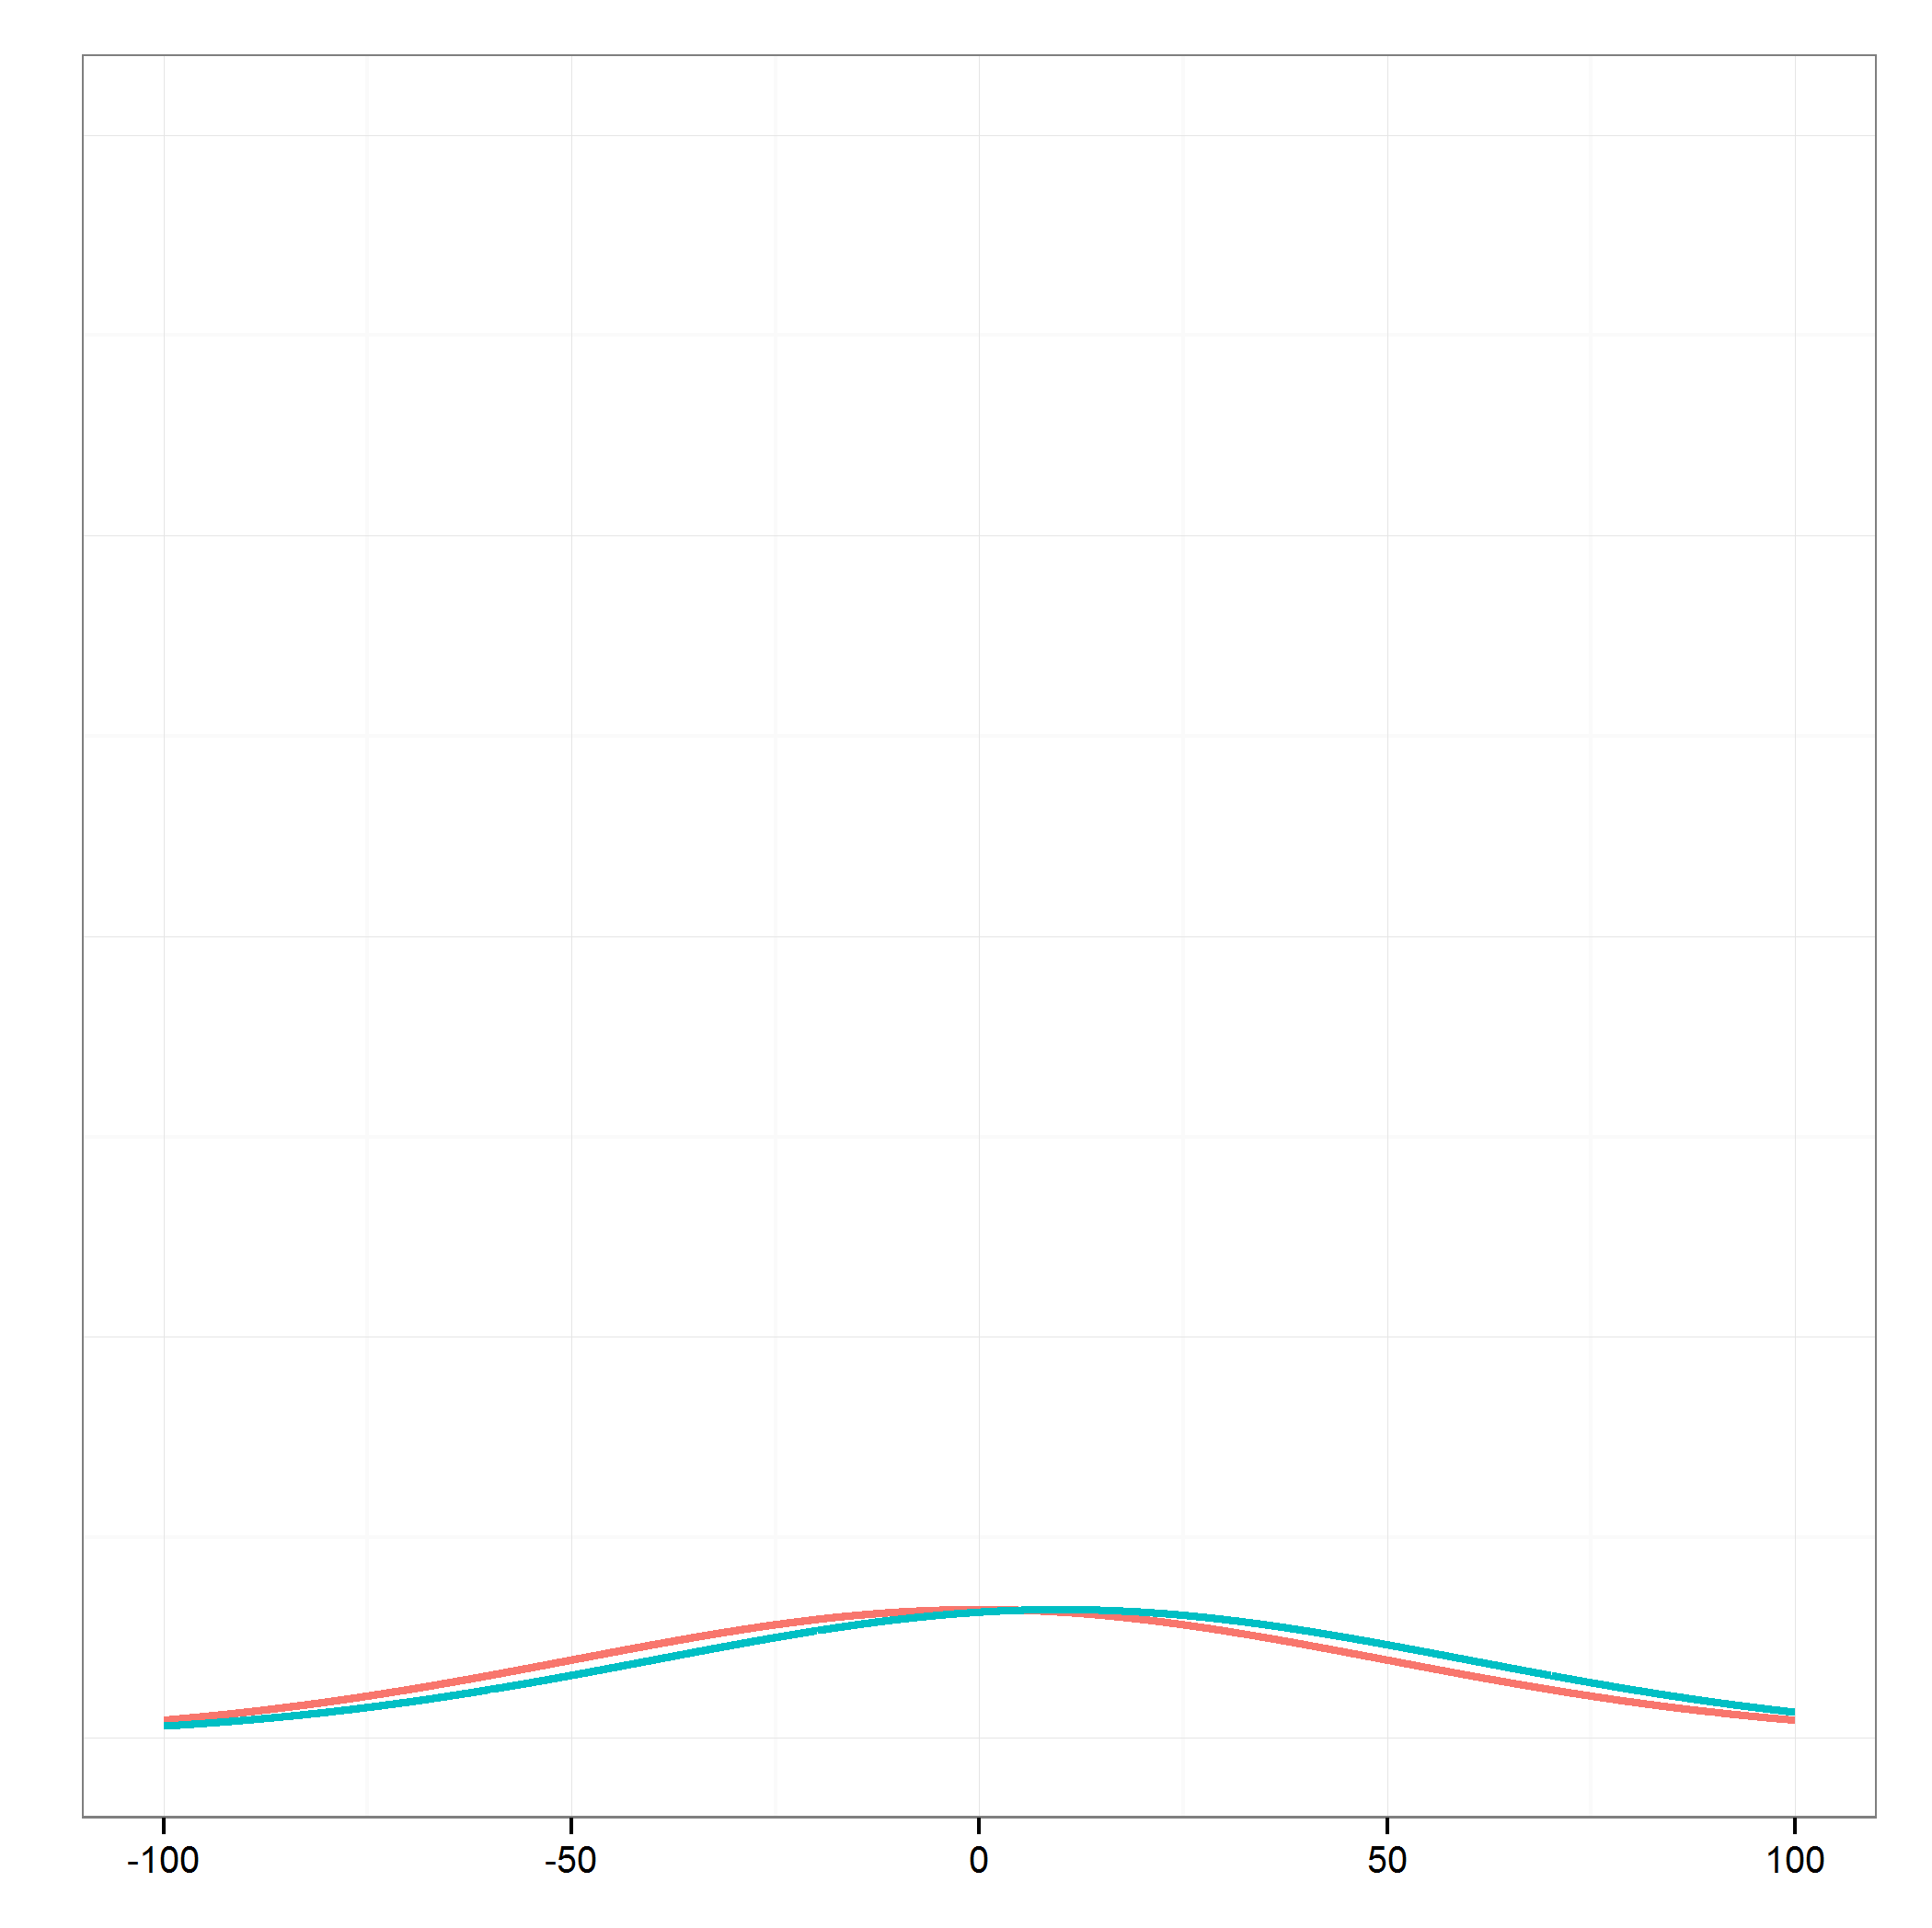
\includegraphics[scale=.3]{figs/first}
\end{block}
\end{column}%
\hfill%
\uncover<2->{
\begin{column}{.48\textwidth}
%\color{blue}\rule{\linewidth}{4pt}
\begin{block}{\small Low Euclidean distance, High Distribution similarity}
{\small
$\mu_1=0,\sigma_1=0.01K$\\
$\mu_2=0.1,\sigma_2=0.01K$
}
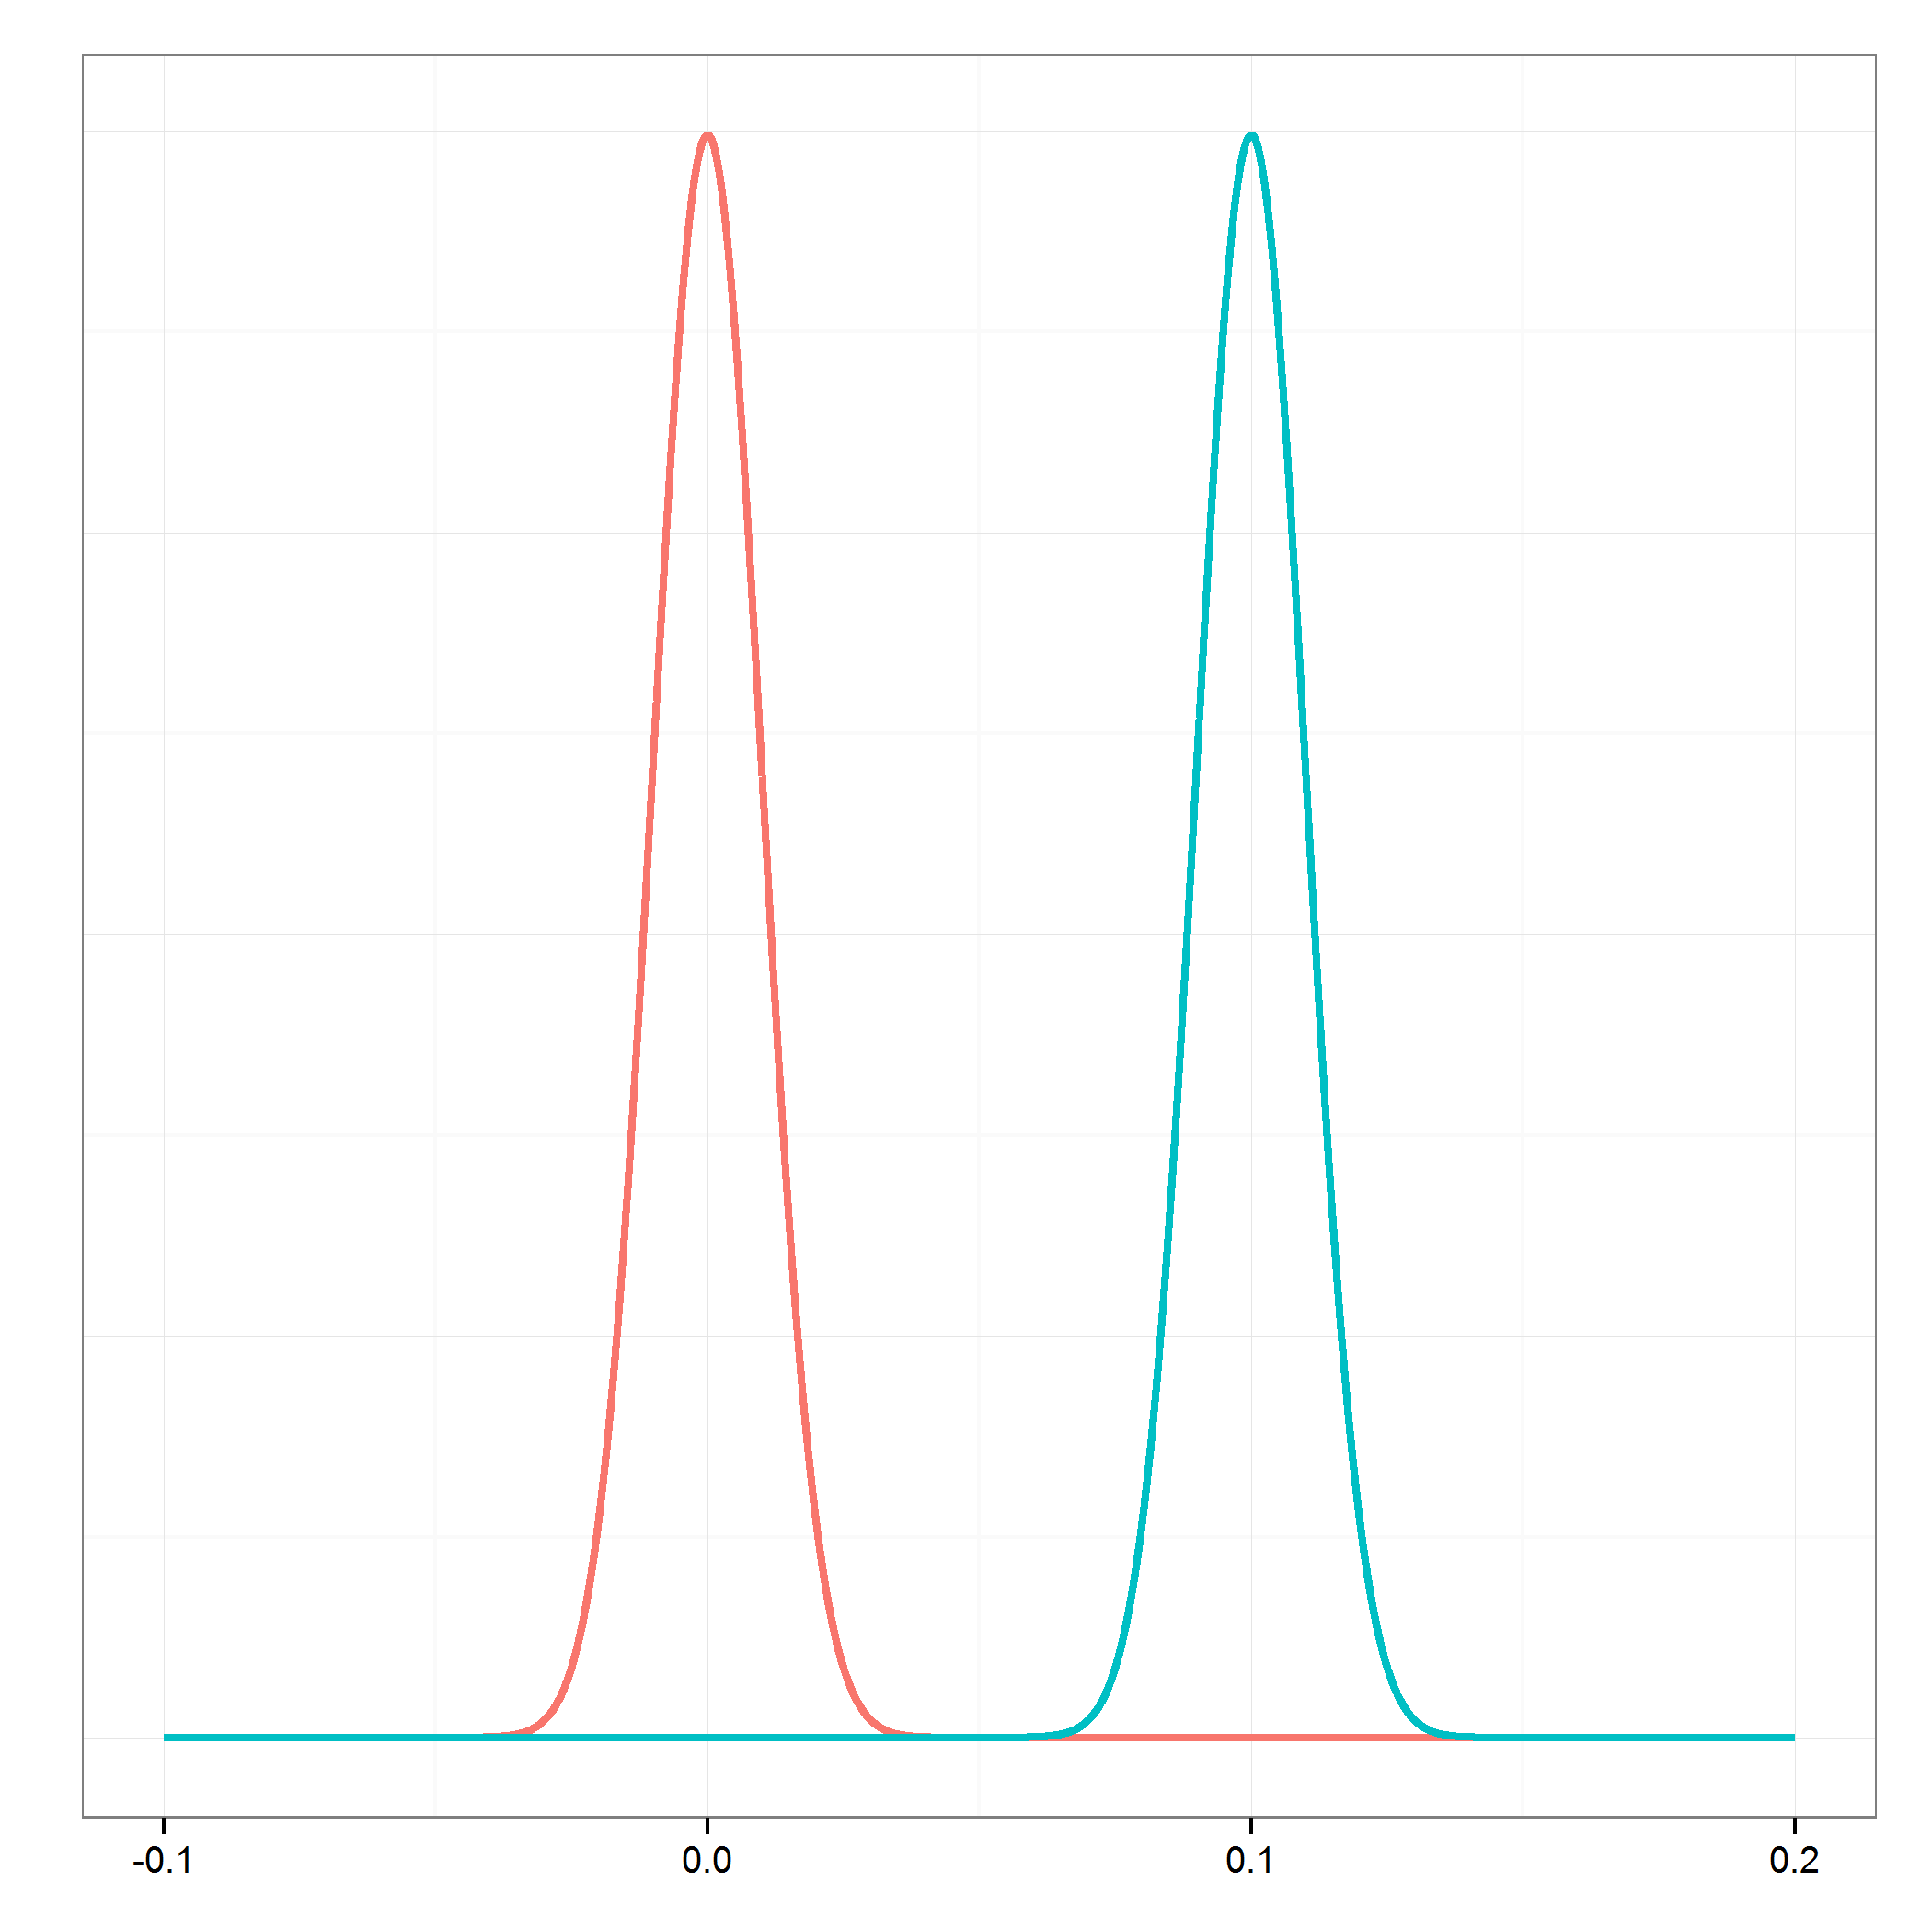
\includegraphics[scale=.3]{figs/second}
\end{block}
\end{column}%
}
\end{columns}
%%%%%%%%%%
}
\frame{\frametitle{Natural Gradient}
 Talk about Natural Gradient
}

\frame{\frametitle{EM vs. Variational Inference}
 Online Variational Inference 4 picture Algorithm Comparison
}

\frame{\frametitle{Local Optimization}
How did we get $\lvp{\phi(\gvp{\lambda})} = \mathbb{E}_{\lambda^{(t-1)}}[\eta_g(x_n,z_{n\backslash j}, \beta)]$?

\begin{enumerate}
\item $\lvp{\phi}(\gvp{\lambda}) = $ \lvp{\text{local}} variational parameters locally optimized given some \gvp{\text{global parameters}}

$$\lvp{\phi}(\gvp{\lambda}) \text{ such that } \nabla_\phi \mathcal{L}(\lambda, \phi(\lambda)) = 0$$
\end{enumerate}
}

\frame{\frametitle{Global Optimization}
\begin{enumerate}
\item If $\mathcal{L}(\lambda) = \mathcal{L}_0(\lambda,\phi(\lambda))$, then 

$$\nabla_\lambda \mathcal{L}(\lambda) = \nabla_\lambda \mathcal{L}_0(\lambda, \phi(\lambda))$$

since $\nabla_\phi \mathcal{L}_0(\lambda, \phi(\lambda)) = 0$
\item<2-> Use chain rule, variational factorization and $\mathcal{L} = D_{KL} + C$ to write 
\begin{eqnarray*}
\mathcal{L} & = &
\mathbb{E}_q[\log p(\beta)] 
- \mathbb{E}_q[\log q(\beta)] \\
& & + \sum_{n=1}^N 
\max_{\phi_n}\left( 
\mathbb{E}_q[\log(x_n,z_n | \beta)] 
- \mathbb{E}_q[\log q(z_n)]
\right)
\end{eqnarray*}
\end{enumerate}
}

\frame{\frametitle{Expectation of Random Function}
\begin{enumerate}
\item We draw an index $I$ u.a.r.
\item<2-> \textit{Define} a random function specific to $I$
\uncover<3-> {
\begin{eqnarray*}
\mathcal{L}_I
&  = &
\mathbb{E}_q[\log p(\beta)] 
- \mathbb{E}_q[\log q(\beta)] \\
& & + N 
\max_{\phi_{\alert{I}}}\left( 
\mathbb{E}_q[\log(x_{\alert{I}},z_{\alert{I}} | \beta)] 
- \mathbb{E}_q[\log q(z_{\alert{I}})]
\right)
\end{eqnarray*}
}
\item<4-> $E_q[\mathcal{L}_I(\lambda)] = \mathcal{L}(\lambda)$
\uncover<5->{$ \Rightarrow \hat\nabla_\lambda \mathcal{L}_I$ is noisy, unbiased estimate of $\hat\nabla_\lambda \mathcal{L}$}
\end{enumerate}
}

\frame{\frametitle{Hallucinating Repetitious Data}
\begin{enumerate}
\item Let's replace original data

$$\{(x_i,z_i)\}_{i=1}^N$$
with $N$ copies of $x_I$:

$$\{(x_I,z_I)\}_{i=1}^N = \left(x_I^{(N)},z_I^{(N)}\right)$$
\item<2-> $\mathcal{L}$ under this data $ = \mathcal{L}_I$
\begin{itemize}
\item<3-> Just use natural gradient formula from before!
\end{itemize}
\item<4-> Calculate localized gradients for each example $i$:
$$\hat\nabla_\lambda \mathcal{L}_i = 
\alpha + N\cdot \left(
	\mathbb{E}_{\phi_{\alert{i}(\lambda)}}[T(x_i,z_i)],
	1
\right) - \lambda$$
\item<5-> Interpolate each local parameter update with the previous iteration's
\end{enumerate}
}

\frame{\frametitle{Schedule}
$\{\rho_t\}$ must satisfy
\begin{itemize}
\item $\sum_t \rho_t = \infty$
\item $\sum_t \rho_t^2 < \infty$
\end{itemize}

Given some \textit{delay} $\tau \ge 0$ and \textit{forgetting rate} $\frac{1}{2} < \kappa \le 1$, set 

$$ \rho_t = \dfrac{1}{(t + \tau)^\kappa}$$
}

\frame{\frametitle{Variational + $x,\; \forall x$}
  \begin{itemize}
    \item Variational EM - the process described above
    \item Variational Bayes - approximate inference (no M-step)
    \item Variational Decoding - approximation decoding 
      
  \end{itemize}

}


\end{document}

